\section{Fault-Tolerance Mechanisms}\label{sec:mechanisms}
Microservices often depend on other microservices in order to
operate correctly. However, it is important to create each
microservice as an independent unit as opposed to viewing it as part
of a bigger system. In order to do so it is essential to design for
failure. All interactions between two microservices must be handled
with care. Assume microservice \emph{A} relies on microservice
\emph{B}. Microservice \emph{A} must be able to react on microservice
\emph{B} being slow or non responding, and it should do so in a timely
manner.
\\\\
This section covers some mechanisms which can improve fault tolerance in
microservice architectures. Their functionality and intended purpose will
be covered in this section, and their implementation will be covered in 
Section~\ref{sec:implementation}.

\subsection{Timeouts}
Microservices are interlinked by nature. Looking at the example
architecture from Section~\ref{sec:architecture} it shows that the
trader service depends on both the account service and the stock
service to function properly. If one of these services are
inaccessible, requests to the trade service must fail and it should
preferably do so quickly.
\\\\
Each request from one service to another takes up a thread from the
thread pool. In the case of the trader service the requests occur
synchronously so only one request is active at a given time, hence
only one extra thread is acquired by one request to the trader
service.
\\\\
If the account service is responding slowly, the trader service will
become slow as well. As trade requests keep coming in, an even greater
pressure is applied to the account service which continues to slow
down. Eventually all threads from the thread pool are busy, yielding an
ever growing queue of incoming requests, slowing down both the account
service and the trader service.
\\\\
If the account service is not responding at all, the trader service
will quickly block all available threads. Once again incoming requests
will be queued and no results are returned.
\\\\
The solution to this is to include timeouts between service
interactions~\cite{avanza} - in this case on all requests from the
trader service to both the account service and the stock service. The
timeouts should be aggressive in order to fail quickly and avoid a
queue building up. If the account service typically replies in 1
second, a timeout of 0.5 seconds would result in virtually no trades
being accepted. However, a timeout of 5 seconds might be too long as
it takes too long to react to the account service failing. Thus, the
timeouts must be set individually for each interaction between
services and it should be such that most requests succeed when all
services function normally and cascading failure is avoided when one
or more services are failing.
 
\subsection{Bulkheads}
Timeouts are essential but they do not cover all cases. If a service
is consistently slow but not slow enough to be caught by the timeout,
all threads get blocked once again and a request queue starts building
up. Bulkheads can be implemented to avoid this.
\\\\
Bulkheads is a general technique where a process is granted access to
only a limited amount of a specific resource. In case of
fault tolerant microservices it can be beneficial to only allow a
limited number of concurrent requests between two services. When the
maximum number of concurrent requests is reached, all incoming
requests are rejected and fail instantly. By doing this a request
queue is never allowed to be created and the called services are
protected from being overloaded~\cite{avanza}.
\\\\
The drawback of this method is that the amount of rejected requests
can become big if the number of allowed concurrent requests is too
conservative. A good bulkhead size can be estimated by inspecting the
number of concurrent requests per second during peak load as well as
the average response time. The sensible bulkhead size would be a
multiplier of these number plus an added buffer to allow for
fluctuations to some degree.

\subsection{Circuit Breaker}
Since microservices typically rely on networked interprocess communication,
there is a risk of calls between them failing or hanging with no timely
response.
If a service relies on another service which starts failing, resulting in not
responding and letting requests hang, the requesting service can waste its
resources on threads waiting for responses. Other than affecting the requesting
services interaction with the failing service, it might also take its resources
from serving its own functionality to other services. This can result in
cascading failures throughout a system~\cite{fowler2014blog}.
Failures can be anything from requests timing out, $5xx HTTP$ responses to
overflowing message queues. 
\newline\newline
The \textit{Circuit Breaker} pattern was introduced by Michael
Nygard~\cite{nygard2007release}, and solves the problem of resource exhaustion
caused by requests to failing services, by failing quickly if it is observed
that requests to a service fail frequently. 
This is achieved by wrapping all calls/requests to a service in a
\textit{circuit breaker} object, which monitors the interaction for continuous
number of failures. 
If the number of failing requests reach some predefined threshold, the circuit
is opened. 
\newline\newline
When in the \textit{open} state, requests will fail immediately instead of being
forwarded, hereby minimizing the number of threads waiting for responses and
allowing the requested service to recover from whatever has caused it to fail.
After some defined timeout, the circuit will transition to a \textit{half-open}
state, where requests will be let through to the service, to see if it functions
again. If it functions as expected, the circuit will be opened again, if not it
will go back to its \textit{closed} state again. This is illustrated as a state
machine in Figure~\ref{fig:circuitbreakerstate}.

\begin{figure}[H]
\centering
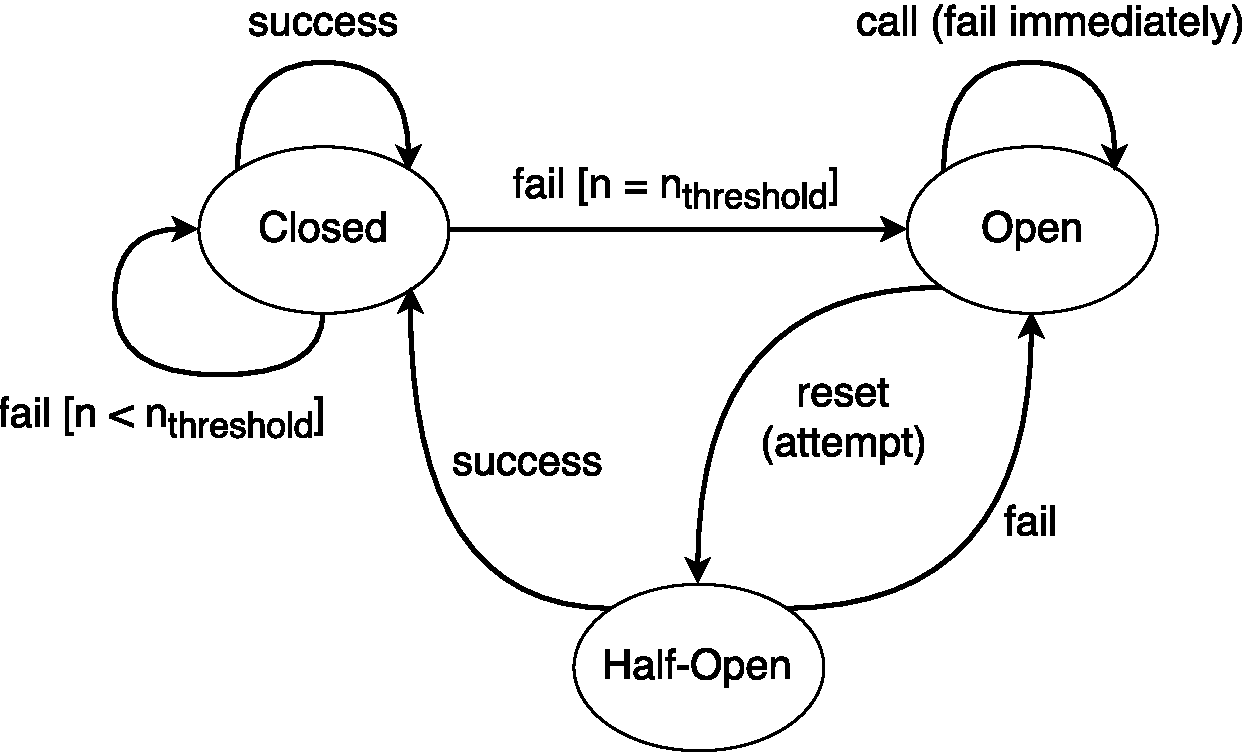
\includegraphics[width=0.7\textwidth]{../media/CircuitBreakerState.pdf} 
\caption{State machine representing the \textit{circuit breaker}. The
	circuit can be in states \textit{closed}, \textit{open} or \textit{half-open}.
	The circuit will transition to its \textit{open} state if number of continuous
	failures reach a predefined threshold. Circuit will be in \textit{closed}
	state until it reaches a timeout where it will reset itself to the
	\textit{half-open} state, from where it will either transition to
	\textit{closed} if a request succeeds or to \textit{open} if a request fails.}
\label{fig:circuitbreakerstate}
\end{figure}

\subsection{Replication}
% Replication of stateless services, split workload
One key principle of microservices, is the componentization of software in
independent services. If they are implemented in a stateless manner, only
persisting state in databases, the independent services can be replicated and
function side-by-side, hereby splitting the system load. Which in many cases
might also minimize errors, since overloading a service could cause faults.
Beyond allowing a service to be scaled horizontally, replication also allows
for increased fault tolerance, since the failure of a single instance does not
necessarily result in breaking the system, since other identical replicated
services are still running. The key goal being that at least one instance of the
service is alive, reachable and well-behaved.
\newline\newline
Replication can be complex if a service holds state, if data needs to be
synchronized across replicated databases or if replicas share resources.
All require a replication strategy that services can base their cooperation on
in order to achieve synchronized state, no corrupted data and no deadlocking or
long waits.
Replication strategies, as covered in the article \textit{The dangers of
replication and a solution}~\cite{gray1996dangers}, might involve solutions
such as timestamps on transactions, \textit{eager} and \textit{lazy} replication
of state across replicas or \textit{master/slave} hierarchies. A strategy should
be chosen based on a systems requirements, types of nodes and data.
In case of the demo system showcased in this report, a simple strategy of
keeping services state-less and using a shared transaction-safe database will
be applied, see Section~\ref{sec:implementation}.
\newline\newline
Replication can enhance fault tolerance even more, if it is applied on a cluster
of servers. Replicating services across a cluster, spreading replicas to
different nodes, lets the system handle sudden disconnects or downtime on
individual nodes. This mentality can even be applied on datacenters and the
cloud, where a single system might run replicated on datacenters and clouds
from different providers and across different regions.
\newline\newline
Another benefit of replication is the ability to deploy a new version of a
service one replica at a time. This allows for evaluation of its performance
in a system and quick rollback if faults are encountered, with no downtime.

\subsection{Redundancy}
% Multiple hosts and services ready for fail-over
Much related to replication is redundancy. Redundancy engineering in general
applies duplicated redundant components ready to take over, if the main
component should fail. Replication offers some sort redundancy, since nodes are
ready to takeover, but all duplicates are active. This is known as
\textit{Active/Active} failover.
\\\\
In \textit{Active/Active} failover, all duplicated nodes function side by side,
and if one fails the other nodes are ready to take over the failed nodes
workload. This might require clients of the failed node to resubmit failed
requests, which then could be handled by the other active nodes. When the failed
node has recovered it can be brought into service again and get its old clients
assigned again.
\\\\
An alternative redundancy failover scheme is \textit{Active/Passive}, where
duplicates are passive until the primary node fails. When the primary node
fails, all resources and clients are transferred to the passive redundant node,
which can resume as the new active primary node. This might also require clients
to resubmit their failed requests. When the failed node comes back online,
either it becomes the new passive node or it is handed its resources and clients
back, making it the active node again with the duplicate redundant node becoming
passive.
